% Author: Daniel Vartanian.
% Licence: MIT. See <https://opensource.org/license/mit/> to learn more.
% Based on: template.tex, developed by the Quarto team and
%   abtex2-modelo-trabalho-academico.tex, v-1.9.7, developed by
%   Lauro César Araujo and the team behind abnt2tex, with additional guidance
%   from the theses and dissertations regulations of the University of São Paulo
%   (USP). For more information, please visit <http://www.abntex.net.br/>.

% For help, see:
% * <https://quarto.org/docs/reference/formats/pdf.html>
% * <https://github.com/abntex/abntex2/wiki/ComoCustomizar>
% * <https://www.ctan.org/pkg/abntex2>
% * <https://www.ctan.org/pkg/memoir>
% * <https://www.ctan.org/pkg/hyperref>

% TODO:
% * Slightly move the toc to the left, in a way that the spacing between titles
%   and numbers become the same as the textual chapters.
% * Remove the hyperlink in the section numbering within TOC.
% * Remove hiperlink spans by page breaks. See: <https://tex.stackexchange.com/questions/54136/hyperref-link-spans-a-pagebreak-looks-ugly>.

% -----
% Preamble
% -----

% Set options for packages loaded elsewhere -----

\PassOptionsToPackage{unicode}{hyperref}
\PassOptionsToPackage{hyphens}{url}
\PassOptionsToPackage{dvipsnames,svgnames,x11names}{xcolor}


% Set \documentclass -----

\documentclass[
12pt,
openright,
oneside,
a4paper,
chapter=TITLE,
section=TITLE,
french,
spanish,
brazil,
english
]{abntex2}
% Load packages -----

\usepackage{array}
\usepackage{booktabs}
\usepackage{calc}
\usepackage{color}
\usepackage{colortbl}
\usepackage{amsmath}
\usepackage{amssymb}
\usepackage{booktabs}
\usepackage{enumitem}
\usepackage{etoolbox}
\usepackage{float}
\usepackage[T1]{fontenc}
\usepackage[hang]{footmisc}
\usepackage{graphicx}
\usepackage{iftex}
\usepackage{indentfirst}
\usepackage[utf8]{inputenc}
\usepackage{lastpage}
\usepackage{lipsum}
\usepackage{longtable}
\usepackage{microtype}
\usepackage{multirow}
\usepackage{parskip}
\usepackage{pdfpages}
\usepackage[table]{xcolor}

\usepackage[
  font=footnotesize,
  justification=centering,
  skip = 1\baselineskip
  ]{caption}

\usepackage{hyperref}

\ifPDFTeX
  \usepackage{textcomp} % provide euro and other symbols
\else % if luatex or xetex
  \usepackage{unicode-math}
\fi

% Set page layout -----

\setlength{\headsep}{1cm}
\setlength{\footskip}{1cm}
\checkandfixthelayout

% Set text -----

\renewcommand{\familydefault}{\sfdefault}

\renewcommand{\baselinestretch}{1.5}

\setlength{\parindent}{1cm}

\setlength{\parskip}{0ex}


\ifPDFTeX\else
    % xetex/luatex font selection
  \setmainfont[]{Arial}
  \setsansfont[]{Arial}
  \setmonofont[ItalicFont=FragmentMono-Italic.otf,Scale=0.75]{FragmentMono-Regular.otf}




\fi


% Set `abntex2` text variables -----

\renewcommand{\ABNTEXchapterfont}{\normalfont\bfseries}
\renewcommand{\ABNTEXchapterfontsize}{\normalsize}
\renewcommand{\ABNTEXsectionfont}{\normalfont}
\renewcommand{\ABNTEXsectionfontsize}{\normalsize}
\renewcommand{\ABNTEXsubsectionfont}{\normalfont\bfseries}
\renewcommand{\ABNTEXsubsectionfontsize}{\normalsize}
\renewcommand{\ABNTEXsubsubsectionfont}{\normalfont}
\renewcommand{\ABNTEXsubsubsectionfontsize}{\normalsize}
\renewcommand{\ABNTEXsubsubsubsectionfont}{\normalfont}
\renewcommand{\ABNTEXsubsubsubsectionfontsize}{\normalsize\itshape}
\renewcommand{\ABNTEXfontereduzida}{\footnotesize}

\renewcommand{\chapnumfont}{\normalfont}
\renewcommand{\captiontitlefont}{\ABNTEXfontereduzida}

\renewcommand{\ABNTEXcaptiondelim}{~\textendash~}
\renewcommand{\ABNTEXcaptionfontedelim}{:~}

% Set page numbering -----

\makepagestyle{abntheadings}
\makeevenhead{abntheadings}{\ABNTEXfontereduzida\thepage}{}{}
\makeoddhead{abntheadings}{}{}{\ABNTEXfontereduzida\thepage}

% Set footnote -----

\setlength{\footnotemargin}{0.5em} % Equal to `\footmarkwidth`
\let\svfootnoterule\footnoterule % Equal to `\footmarksep`
\renewcommand\footnoterule{\svfootnoterule\vspace{1ex}}

% Set language patterns -----

\newcommand{\capaname}{Capa}
\newcommand{\listadetermosname}{Lista de termos e definições}

\addto\captionsenglish{
  \renewcommand{\capaname}{Cover}
  \renewcommand{\folhadeaprovacaoname}{Approval sheet}
  \renewcommand{\dedicatorianame}{Inscription}
  \renewcommand{\contentsname}{Contents}
  \renewcommand{\listfigurename}{List of figures}
  \renewcommand{\listtablename}{List of tables}
  \renewcommand{\listadetermosname}{List of terms and definitions}
}

\addto\captionsbrazil{
  \renewcommand{\capaname}{Capa}
  \renewcommand{\contentsname}{Sumário}
  \renewcommand{\listfigurename}{Lista de figuras}
  \renewcommand{\listadetermosname}{Lista de termos e definições}
}

\addto\captionsspanish{
  \renewcommand{\capaname}{Portada}
  \renewcommand{\folhaderostoname}{Página de título}
  \renewcommand{\epigraphname}{Epígrafe}
  \renewcommand{\dedicatorianame}{Dedicatoria}
  \renewcommand{\errataname}{Errata}
  \renewcommand{\agradecimentosname}{Agradecimientos}
  \renewcommand{\anexoname}{Anexo}
  \renewcommand{\anexosname}{Anexos}
  \renewcommand{\apendicename}{Apéndice}
  \renewcommand{\apendicesname}{Apéndices}
  \renewcommand{\orientadorname}{Asesor:}
  \renewcommand{\coorientadorname}{Coasesor:}
  \renewcommand{\folhadeaprovacaoname}{Hoja de aprobación}
  \renewcommand{\resumoname}{Resumen}
  \renewcommand{\contentsname}{Sumario}
  \renewcommand{\listfigurename}{Lista de figuras}
  \renewcommand{\listtablename}{Lista de tablas}
  \renewcommand{\listadesiglasname}{Lista de abreviaturas y siglas}
  \renewcommand{\listadesimbolosname}{Lista de símbolos}
  \renewcommand{\listadetermosname}{Lista de términos y definiciones}
  \renewcommand{\contentsname}{Sumario}
  \renewcommand{\bibname}{Referencias}
  \renewcommand{\indexname}{Índice}
  \renewcommand{\sourcename}{Fuente}
  \renewcommand{\notaname}{Nota}
  \renewcommand{\pageautorefname}{página}
  \renewcommand{\sectionautorefname}{sección}
  \renewcommand{\subsectionautorefname}{subsección}
  \renewcommand{\subsubsectionautorefname}{subsubsección}
  \renewcommand{\paragraphautorefname}{subsubsubsección}
}

\addto\captionsfrench{
  \renewcommand{\capaname}{Page de titre}
  \renewcommand{\folhaderostoname}{Page de titre}
  \renewcommand{\epigraphname}{Épigraphe}
  \renewcommand{\dedicatorianame}{Dédiace}
  \renewcommand{\errataname}{Errata}
  \renewcommand{\agradecimentosname}{Remerciements}
  \renewcommand{\anexoname}{Annexe}
  \renewcommand{\anexosname}{Annexes}
  \renewcommand{\apendicename}{Appendice}
  \renewcommand{\apendicesname}{Appendices}
  \renewcommand{\orientadorname}{Conseiller :}
  \renewcommand{\coorientadorname}{Co-conseiller :}
  \renewcommand{\folhadeaprovacaoname}{Feuille d'approbation}
  \renewcommand{\resumoname}{Résumé}
  \renewcommand{\contentsname}{Sommaire}
  \renewcommand{\listfigurename}{Liste des figures}
  \renewcommand{\listtablename}{Liste des tableaux}
  \renewcommand{\listadesiglasname}{Liste des abréviations et sigles}
  \renewcommand{\listadesimbolosname}{Liste des symboles}
  \renewcommand{\listadetermosname}{Liste des termes et définitions}
  \renewcommand{\contentsname}{Sommaire}
  \renewcommand{\bibname}{Références}
  \renewcommand{\indexname}{Index}
  \renewcommand{\sourcename}{Source}
  \renewcommand{\notaname}{Note}
  \renewcommand{\pageautorefname}{page}
  \renewcommand{\sectionautorefname}{section}
  \renewcommand{\subsectionautorefname}{sous-section}
  \renewcommand{\subsubsectionautorefname}{sous-sous-section}
  \renewcommand{\paragraphautorefname}{sous-sous-sous-section}
}

% Set other general formatting -----

% Use upquote if available, for straight quotes in verbatim environments
\IfFileExists{upquote.sty}{\usepackage{upquote}}{}
\IfFileExists{microtype.sty}{% use microtype if available
  \usepackage[]{microtype}
  \UseMicrotypeSet[protrusion]{basicmath} % disable protrusion for tt fonts
}{}





\setlength{\emergencystretch}{3em} % Prevent overfull lines

\setcounter{secnumdepth}{5}

% Make \paragraph and \subparagraph free-standing
\ifx\paragraph\undefined\else
  \let\oldparagraph\paragraph
  \renewcommand{\paragraph}[1]{\oldparagraph{#1}\mbox{}}
\fi
\ifx\subparagraph\undefined\else
  \let\oldsubparagraph\subparagraph
  \renewcommand{\subparagraph}[1]{\oldsubparagraph{#1}\mbox{}}
\fi

% Set pandoc -----

\usepackage{color}
\usepackage{fancyvrb}
\newcommand{\VerbBar}{|}
\newcommand{\VERB}{\Verb[commandchars=\\\{\}]}
\DefineVerbatimEnvironment{Highlighting}{Verbatim}{commandchars=\\\{\}}
% Add ',fontsize=\small' for more characters per line
\usepackage{framed}
\definecolor{shadecolor}{RGB}{241,243,245}
\newenvironment{Shaded}{\begin{snugshade}}{\end{snugshade}}
\newcommand{\AlertTok}[1]{\textcolor[rgb]{0.68,0.00,0.00}{#1}}
\newcommand{\AnnotationTok}[1]{\textcolor[rgb]{0.37,0.37,0.37}{#1}}
\newcommand{\AttributeTok}[1]{\textcolor[rgb]{0.40,0.45,0.13}{#1}}
\newcommand{\BaseNTok}[1]{\textcolor[rgb]{0.68,0.00,0.00}{#1}}
\newcommand{\BuiltInTok}[1]{\textcolor[rgb]{0.00,0.23,0.31}{#1}}
\newcommand{\CharTok}[1]{\textcolor[rgb]{0.13,0.47,0.30}{#1}}
\newcommand{\CommentTok}[1]{\textcolor[rgb]{0.37,0.37,0.37}{#1}}
\newcommand{\CommentVarTok}[1]{\textcolor[rgb]{0.37,0.37,0.37}{\textit{#1}}}
\newcommand{\ConstantTok}[1]{\textcolor[rgb]{0.56,0.35,0.01}{#1}}
\newcommand{\ControlFlowTok}[1]{\textcolor[rgb]{0.00,0.23,0.31}{#1}}
\newcommand{\DataTypeTok}[1]{\textcolor[rgb]{0.68,0.00,0.00}{#1}}
\newcommand{\DecValTok}[1]{\textcolor[rgb]{0.68,0.00,0.00}{#1}}
\newcommand{\DocumentationTok}[1]{\textcolor[rgb]{0.37,0.37,0.37}{\textit{#1}}}
\newcommand{\ErrorTok}[1]{\textcolor[rgb]{0.68,0.00,0.00}{#1}}
\newcommand{\ExtensionTok}[1]{\textcolor[rgb]{0.00,0.23,0.31}{#1}}
\newcommand{\FloatTok}[1]{\textcolor[rgb]{0.68,0.00,0.00}{#1}}
\newcommand{\FunctionTok}[1]{\textcolor[rgb]{0.28,0.35,0.67}{#1}}
\newcommand{\ImportTok}[1]{\textcolor[rgb]{0.00,0.46,0.62}{#1}}
\newcommand{\InformationTok}[1]{\textcolor[rgb]{0.37,0.37,0.37}{#1}}
\newcommand{\KeywordTok}[1]{\textcolor[rgb]{0.00,0.23,0.31}{#1}}
\newcommand{\NormalTok}[1]{\textcolor[rgb]{0.00,0.23,0.31}{#1}}
\newcommand{\OperatorTok}[1]{\textcolor[rgb]{0.37,0.37,0.37}{#1}}
\newcommand{\OtherTok}[1]{\textcolor[rgb]{0.00,0.23,0.31}{#1}}
\newcommand{\PreprocessorTok}[1]{\textcolor[rgb]{0.68,0.00,0.00}{#1}}
\newcommand{\RegionMarkerTok}[1]{\textcolor[rgb]{0.00,0.23,0.31}{#1}}
\newcommand{\SpecialCharTok}[1]{\textcolor[rgb]{0.37,0.37,0.37}{#1}}
\newcommand{\SpecialStringTok}[1]{\textcolor[rgb]{0.13,0.47,0.30}{#1}}
\newcommand{\StringTok}[1]{\textcolor[rgb]{0.13,0.47,0.30}{#1}}
\newcommand{\VariableTok}[1]{\textcolor[rgb]{0.07,0.07,0.07}{#1}}
\newcommand{\VerbatimStringTok}[1]{\textcolor[rgb]{0.13,0.47,0.30}{#1}}
\newcommand{\WarningTok}[1]{\textcolor[rgb]{0.37,0.37,0.37}{\textit{#1}}}

\providecommand{\tightlist}{
\setlength{\itemsep}{0pt}\setlength{\parskip}{0pt}}% Correct order of tables after \paragraph or \subparagraph
\usepackage{etoolbox}
\makeatletter
\patchcmd\longtable{\par}{\if@noskipsec\mbox{}\fi\par}{}{}
\makeatother

% Allow footnotes in longtable head/foot
\IfFileExists{footnotehyper.sty}{\usepackage{footnotehyper}}{\usepackage{footnote}}
\makesavenoteenv{longtable}% \usepackage{graphicx}
\makeatletter
\def\maxwidth{\ifdim\Gin@nat@width>\linewidth\linewidth\else\Gin@nat@width\fi}
\def\maxheight{\ifdim\Gin@nat@height>\textheight\textheight\else\Gin@nat@height\fi}
\makeatother

% Scale images if necessary, so that they will not overflow the page
% margins by default, and it is still possible to overwrite the defaults
% using explicit options in \includegraphics[width, height, ...]{}
\setkeys{Gin}{width=\maxwidth,height=\maxheight,keepaspectratio}

% Set default figure placement to htbp
\makeatletter
\def\fps@figure{htbp}
\makeatother

%:::% class attribute begin/end %:::%

% -----
% Title page
% -----

%:::% title-page begin %:::%
\preambulo{
%:::% title-page body begin %:::%
\imprimirnotadeversao
\vspace{1.5em}

{\imprimirtipotrabalho} presented to the {\imprimirescola} at {\imprimiruniversidade}, as part of the requirements for the degree of {\imprimirtituloacademico} by the {\imprimirprograma}.
\vspace{1em}

Area of concentration: {\imprimirareadeconcentracao}.
\vspace{1em}

Revised version incorporating the changes requested by the examining committee on [Date]. The original version is held in the reserved collection at the {\imprimirescola} Library and in the Digital Library of Theses and Dissertations of the {\imprimiruniversidade}.
\vspace{1em}

Supervisor: Prof. Dr. {\imprimirorientador}
\vspace{0.5em}

Co-Supervisor: Prof. Dr. {\imprimircoorientador}
%:::% title-page body end %:::%
}
%:::% title-page end %:::%
\usepackage{booktabs}
\usepackage{caption}
\usepackage{longtable}
\usepackage{colortbl}
\usepackage{array}
\makeatletter
\@ifpackageloaded{tcolorbox}{}{\usepackage[skins,breakable]{tcolorbox}}
\@ifpackageloaded{fontawesome5}{}{\usepackage{fontawesome5}}
\definecolor{quarto-callout-color}{HTML}{909090}
\definecolor{quarto-callout-note-color}{HTML}{0758E5}
\definecolor{quarto-callout-important-color}{HTML}{CC1914}
\definecolor{quarto-callout-warning-color}{HTML}{EB9113}
\definecolor{quarto-callout-tip-color}{HTML}{00A047}
\definecolor{quarto-callout-caution-color}{HTML}{FC5300}
\definecolor{quarto-callout-color-frame}{HTML}{acacac}
\definecolor{quarto-callout-note-color-frame}{HTML}{4582ec}
\definecolor{quarto-callout-important-color-frame}{HTML}{d9534f}
\definecolor{quarto-callout-warning-color-frame}{HTML}{f0ad4e}
\definecolor{quarto-callout-tip-color-frame}{HTML}{02b875}
\definecolor{quarto-callout-caution-color-frame}{HTML}{fd7e14}
\makeatother
\makeatletter
\makeatother
\makeatletter
\@ifpackageloaded{bookmark}{}{\usepackage{bookmark}}
\makeatother
\makeatletter
\@ifpackageloaded{caption}{}{\usepackage{caption}}
\AtBeginDocument{%
\ifdefined\contentsname
  \renewcommand*\contentsname{Table of contents}
\else
  \newcommand\contentsname{Table of contents}
\fi
\ifdefined\listfigurename
  \renewcommand*\listfigurename{List of Figures}
\else
  \newcommand\listfigurename{List of Figures}
\fi
\ifdefined\listtablename
  \renewcommand*\listtablename{List of Tables}
\else
  \newcommand\listtablename{List of Tables}
\fi
\ifdefined\figurename
  \renewcommand*\figurename{Figure}
\else
  \newcommand\figurename{Figure}
\fi
\ifdefined\tablename
  \renewcommand*\tablename{Table}
\else
  \newcommand\tablename{Table}
\fi
}
\@ifpackageloaded{float}{}{\usepackage{float}}
\floatstyle{ruled}
\@ifundefined{c@chapter}{\newfloat{codelisting}{h}{lop}}{\newfloat{codelisting}{h}{lop}[chapter]}
\floatname{codelisting}{Listing}
\newcommand*\listoflistings{\listof{codelisting}{List of Listings}}
\makeatother
\makeatletter
\@ifpackageloaded{caption}{}{\usepackage{caption}}
\@ifpackageloaded{subcaption}{}{\usepackage{subcaption}}
\makeatother
\makeatletter
\@ifpackageloaded{tcolorbox}{}{\usepackage[skins,breakable]{tcolorbox}}
\makeatother
\makeatletter
\@ifundefined{shadecolor}{\definecolor{shadecolor}{HTML}{CFD0D1}}
\makeatother
\makeatletter
\@ifundefined{codebgcolor}{\definecolor{codebgcolor}{HTML}{F1F3F5}}
\makeatother
\makeatletter
\makeatother

% Set new commands -----

\providecommand{\imprimiruniversidade}{}
\newcommand{\universidade}[1]{\renewcommand{\imprimiruniversidade}{#1}}

\providecommand{\imprimirescola}{}
\newcommand{\escola}[1]{\renewcommand{\imprimirescola}{#1}}

\providecommand{\imprimirprograma}{}
\newcommand{\programa}[1]{\renewcommand{\imprimirprograma}{#1}}

\newcommand{\imprimirtipodetrabalho}{\imprimirtipotrabalho}

\providecommand{\imprimirtipodetituloacademico}{}
\newcommand{\tipodetituloacademico}[1]{\renewcommand{\imprimirtipodetituloacademico}{#1}}

\providecommand{\imprimirtituloacademico}{}
\newcommand{\tituloacademico}[1]{\renewcommand{\imprimirtituloacademico}{#1}}

\providecommand{\imprimirareadeconcentracao}{}
\newcommand{\areadeconcentracao}[1]{\renewcommand{\imprimirareadeconcentracao}{#1}}

\providecommand{\imprimirnotadeversao}{}
\newcommand{\notadeversao}[1]{\renewcommand{\imprimirnotadeversao}{#1}}

\makeatletter
\newcommand*{\getlength}[1]{\strip@pt#1}
\makeatother

% Set title variables -----

\title{\{abnt\}: Quarto format for ABNT theses and dissertations}
\titulo{\{abnt\}: Quarto format for ABNT theses and dissertations}


\author{Daniel Vartanian}
\autor{Daniel Vartanian}

\local{{[}City{]}}

\date{2023}
\data{2023}

\orientador{{[}Supervisor's full name{]}}

\coorientador{{[}Co-supervisor's full name{]}}

\tipodetituloacademico{{[}Master/PhD{]}}

\tituloacademico{{[}Master of Science/Doctor of Science{]}}

\tipotrabalho{{[}Dissertation/Thesis{]}}

\areadeconcentracao{{[}Area of concentration{]}}

\instituicao{\MakeUppercase{{[}University{]}}}
\universidade{{[}University{]}}

\instituicao{
  \MakeUppercase{{[}University{]}}
  \par
  \MakeUppercase{{[}School/Department{]}}
}

\escola{{[}School/Department{]}}

\instituicao{
  \MakeUppercase{{[}University{]}}
  \par
  \MakeUppercase{{[}School/Department{]}}
  \par
  \MakeUppercase{{[}Graduate program{]}}
}

\programa{{[}Graduate program{]}}

\notadeversao{{[}Original/Revised version{]}}

% Set hipersetup -----

\hypersetup{
pdftitle={\{abnt\}: Quarto format for ABNT theses and dissertations},
pdfauthor={Daniel Vartanian},
pdflang={en},
pdfsubject={{[}Dissertation/Thesis{]}},
linktoc={section},
colorlinks=true,
linkcolor={blue},
filecolor={blue},
citecolor={blue},
urlcolor={blue},
pdfcreator={LaTeX via pandoc},
bookmarksdepth=5
}

% Set chapter/section formating -----

\setsecnumformat{\normalfont\csname the#1\endcsname\quad}

\renewcommand{\printchapternum}{
  \tocprintchapter
  \setboolean{abntex@innonumchapter}{false}
  \chapnumfont
  \thechapter \quad
  \ifthenelse{\boolean{abntex@apendiceousecao}}{
      \tocinnonumchapter
      \ABNTEXcaptiondelim
  }{}
}

\setlength{\beforechapskip}{2.5em}
\setlength{\afterchapskip}{1em}
\setbeforesecskip{1.5em}
\setaftersecskip{1em}
\setbeforesubsecskip{1.5em}
\setaftersubsecskip{1em}
\setbeforesubsubsecskip{1.5em}
\setaftersubsubsecskip{1em}
\setbeforeparaskip{1.5em}
\setafterparaskip{0em} % check
\setparahook{\vspace{1.5em}}

% Set tabular environment -----

% \providecommand{\addquartolegend}{}
% \newcommand{\quartolegend}[1]{\renewcommand{\addquartolegend}{#1}}
% \renewcommand{\quartolegend}{Don't forget to set \verb|\quartolegend|!}

\AtBeginEnvironment{table}{\ABNTEXfontereduzida}
\AtBeginEnvironment{tabular}{\ABNTEXfontereduzida}
\renewcommand{\arraystretch}{1.5}
\setlength{\aboverulesep}{0ex}
\setlength{\belowrulesep}{0ex}

\AddToHook{env/longtable/before}{}
\AddToHook{env/longtable/after}{}
\AddToHook{env/longtable/begin}{
  \ABNTEXfontereduzida
  \renewcommand{\arraystretch}{1.5}
  \legend{test}
}
\AddToHook{env/longtable/end}{}

% Set figure environment -----

\makeatletter
\setlength{\@fptop}{5pt} % Set distance from top of page to first float
\makeatother

\renewcommand{\legend}[1]{
  \vspace*{1\baselineskip}
  \ABNTEXfontereduzida \raggedright #1
  \vspace{1.5\baselineskip}
}

% % Credits: <https://stackoverflow.com/a/1566053/8258804>.
% \makeatletter
% \let\oldfigure\figure
% \def\figure{\@ifnextchar[\figure@i \figure@ii}
% \def\figure@i[#1]{\oldfigure[#1]\centering}
% \def\figure@ii{\oldfigure\centering}
% \makeatother

% Change `abntex2` commands and enviroments -----


% Similar to \printloftitle
\renewcommand{\pretextualchapter}[1]{
  \setlength{\afterchapskip}{4.5em}
  \addtocounter{abntex@bookmarkcounter}{1}
  \PRIVATEbookmarkthis{#1}
  \chapter*[#1]{#1}
}

\renewcommand{\textual}{
  \pagestyle{abntheadings}
  \aliaspagestyle{chapter}{abntheadings}
}

\renewcommand{\imprimircapa}{
  \phantomsection\pdfbookmark[0]{\capaname}{}
  \begin{capa}%
  \begin{adjustwidth}{-1cm}{0cm}
  \center
  \imprimirinstituicao
  \vfill

  \imprimirautor
  \vfill

  \textbf{\imprimirtitulo}
  \vspace{10cm}

  \imprimirlocal

  \imprimirdata
  \vspace*{1.5cm}
  \end{adjustwidth}
  \end{capa}
}

\makeatletter
\renewcommand{\folhaderostocontent}{
  \begin{center}
  \imprimirautor
  \vfill

  \textbf{\imprimirtitulo}
  \vfill

  \abntex@ifnotempty{
    \imprimirpreambulo
  }{
    \hspace{0.35\textwidth}
    \begin{minipage}{.6\textwidth} % page width
    \SingleSpacing
    \imprimirpreambulo
    \end{minipage}
    \vfill
  }

  \imprimirlocal

  \imprimirdata
  \vspace*{1cm}
  \end{center}
}
\makeatother

\renewenvironment{fichacatalografica}{
  \ABNTEXfontereduzida
  \setlength{\parindent}{0cm}
  \begin{SingleSpacing}
}{
  \end{SingleSpacing}%
}

\renewenvironment{siglas}{
  \pretextualchapter{\listadesiglasname}
}{
  \cleardoublepage
}

\renewenvironment{simbolos}{
  \pretextualchapter{\listadesimbolosname}
}{
  \cleardoublepage
}

\newenvironment{termos}{%
  \pretextualchapter{\listadetermosname}
}{
  \cleardoublepage
}

\newenvironment{resumoenv}[1][\resumoname]{
  \pretextualchapter{#1}
  \setlength{\parindent}{0cm}
  \setlength{\parskip}{1em}
  \AtBeginEnvironment{tabular}{\normalsize}
  \renewcommand{\arraystretch}{1}
  \setlength{\aboverulesep}{0em}
  \setlength{\belowrulesep}{0em}
  \setlength{\arrayrulewidth}{0em}
  \setlength{\tabcolsep}{0em}
  \begin{SingleSpace}
}{
  \end{SingleSpace}
  \clearpage
}

\makechapterstyle{apendice}{
  \setlength{\beforechapskip}{-\baselineskip}
  \setlength{\midchapskip}{0em}
  \setlength{\afterchapskip}{1em}
  \renewcommand{\chapnamefont}{\normalfont}
  \renewcommand{\printchaptername}{\ABNTEXchapterupperifneeded{\appendixname}}
  \renewcommand{\chapternamenum}{\space}
  \renewcommand{\chapnumfont}{\normalfont}
  \renewcommand{\printchapternum}{\thechapter}
  \renewcommand{\afterchapternum}{\space -- \space}
  \renewcommand{\chaptitlefont}{\normalfont}
  \renewcommand{\printchaptertitle}[1]{\ABNTEXchapterupperifneeded{##1}}
  \renewcommand{\afterchaptertitle}{\vspace{1em}}
}

\renewcommand{\PRIVATEapendiceconfig}[1]{
  \setboolean{abntex@apendiceousecao}{true}
  \renewcommand{\appendixname}{#1}
  \renewcommand{\apendicesname}{#1}
  \switchchapname{#1}

  % Note:
  %
  % \cleardoublepage
  % \phantomsection
  % \addcontentsline{toc}{part}{Appendices}
  % \appendix
  %
  % is automatically add by the Quarto render.
}

\newcommand{\PRIVATEannexconfig}[2]{
  \setboolean{abntex@apendiceousecao}{true}
  \renewcommand{\appendixname}{#1}
  \renewcommand{\apendicesname}{#1}
  \renewcommand{\appendixtocname}{#2}
  \phantomsection
  \addcontentsline{toc}{part}{\appendixtocname}
  \switchchapname{#1}
}

\renewcommand{\apendices}{
  \cftinserthook{toc}{appendixhook}
  \PRIVATEapendiceconfig{\apendicename}
  \appendix
  \chapterstyle{apendice}
}

\renewenvironment{apendicesenv}{
  \cftinserthook{toc}{appendixhook}
  \PRIVATEapendiceconfig{\apendicename}
  \begin{appendix}
  \chapterstyle{apendice}
}{
  \end{appendix}
  \setboolean{abntex@apendiceousecao}{false}
  \bookmarksetup{startatroot}
}

\renewcommand{\anexos}{
  \cftinserthook{toc}{appendixhook}
  \PRIVATEannexconfig{\anexoname}{\anexosname}
  \appendix
  \renewcommand\theHchapter{anexochapback.\arabic{chapter}}
  \chapterstyle{apendice}
}

\renewenvironment{anexosenv}{
  \cftinserthook{toc}{appendixhook}
  \PRIVATEannexconfig{\anexoname}{\anexosname}
  \begin{appendix}
  \renewcommand\theHchapter{anexochapback.\arabic{chapter}}
  \chapterstyle{apendice}
}{
  \end{appendix}
  \setboolean{abntex@apendiceousecao}{false}
  \bookmarksetup{startatroot}
}

% Set LoF & LoT -----

\renewcommand{\printloftitle}[1]{
  \setlength{\afterchapskip}{2.3em}
  \chapter*[#1]{#1}
}

\renewcommand{\printlottitle}[1]{
  \setlength{\afterchapskip}{2.3em}
  \chapter*[#1]{#1}
}

% Set ToC -----

\renewcommand{\aftertoctitle}{\center\vspace{3em}}

\setlength{\cftpartindent}{6em}
\setlength{\cftsectionnumwidth}{6em}
\setlength{\cftsubsectionnumwidth}{6em}
\setlength{\cftsubsubsectionnumwidth}{6em}
\setlength{\cftparagraphnumwidth}{6em}

\setlength{\cftbeforebookskip}{0pt}
\setlength{\cftbeforepartskip}{2em}
\setlength{\cftbeforechapterskip}{0.5em}
\setlength{\cftbeforesectionskip}{0pt}
\setlength{\cftbeforesubsectionskip}{0pt}
\setlength{\cftbeforesubsubsectionskip}{0pt}
\setlength{\cftbeforeparagraphskip}{0pt}

\renewcommand{\cftchapterpresnum}{\normalfont}
\renewcommand{\cftchapteraftersnum}{\normalfont}
\renewcommand{\cftchapteraftersnumb}{\normalfont\normalsize\bfseries\hspace{0.87em}}
\renewcommand{\cftsubsectionpresnum}{\normalfont}
\renewcommand{\cftparagraphpresnum}{\normalfont}

\renewcommand{\cftpartfont}{\normalfont\normalsize\bfseries\MakeUppercase}
\renewcommand{\cftchapterfont}{\normalfont\normalsize\bfseries\MakeUppercase}
\renewcommand{\cftsectionfont}{\normalfont\normalsize\MakeUppercase}
\renewcommand{\cftsubsectionfont}{\normalfont\normalsize\bfseries}
\renewcommand{\cftsubsubsectionfont}{\normalfont\normalsize}
\renewcommand{\cftparagraphfont}{\normalfont\normalsize\itshape}

\renewcommand{\cftpartpagefont}{\normalfont\normalsize}
\renewcommand{\cftchapterpagefont}{\normalfont\normalsize}
\renewcommand{\cftsectionpagefont}{\normalfont\normalsize}
\renewcommand{\cftsubsectionpagefont}{\normalfont\normalsize}
\renewcommand{\cftsubsubsectionpagefont}{\normalfont\normalsize}
\renewcommand{\cftparagraphpagefont}{\normalfont\normalsize}
\renewcommand{\cftfigurepagefont}{\normalfont\normalsize}
\renewcommand{\cfttablepagefont}{\normalfont\normalsize}

\cftinsertcode{bibhook}{
  \setlength{\cftchapterindent}{5.675em}
  \setlength{\cftchapternumwidth}{0em}
  \renewcommand{\cftchapteraftersnumb}{\hspace{0em}}
  \renewcommand{\cftchapterpresnum}{\normalfont\bfseries}
}

\cftinsertcode{appendixhook}{
    \setlength{\cftchapterindent}{6em} %
    \renewcommand{\cftchaptername}{\appendixname\space}
    \setlength{\cftchapternumwidth}{2.3em} % check
    \renewcommand{\cftchapteraftersnumb}{
        \hspace{-1.5em} -- \space % check \hspace{-1.5em}
    }
}
% Set bibliography -----

\renewcommand{\bibname}{REFERENCES}
\newcommand{\newbibname}{REFERENCES}

\newcommand{\bibnamewithfootnote}{
  REFERENCES\protect\footnote{In accordance with ABNT style -- Brazilian
Association of Technical Standards.}
}

\usepackage[
style=abnt,backend=biber,,language=english,,url=true,,useprefix=false,,giveninits=true,,extrayear=true]{biblatex}
\usepackage{csquotes}
\addbibresource{references.bib}

\defbibheading{bay}[\bibnamewithfootnote]{
  \ifthenelse{\boolean{ABNTEXupperchapter}}{
    \setboolean{ABNTEXupperchapter}{false}
    \chapter*{#1}
    \markboth{#1}{#1}
    \setboolean{ABNTEXupperchapter}{true}
  }{
    \chapter*{#1}
    \markboth{#1}{#1}
  }
}

\AtBeginBibliography{\vspace{4em}}
\AtEveryBibitem{\clearfield{annotation}}
\renewcommand{\bibfont}{\ABNTEXfontereduzida}

\setlength{\bibhang}{0cm}

\setlength{\bibparsep}{0ex}


% Set colors -----

\definecolor{blue}{HTML}{2905C3}

% See <https://getbootstrap.com/docs/4.0/utilities/colors/>.
\definecolor{quarto-blue}{HTML}{2780E3}
\definecolor{quarto-lighter-blue}{HTML}{ECF4FC}
\definecolor{quarto-orange}{HTML}{FF7518}
\definecolor{quarto-ligther-orange}{HTML}{FFF3EB}
\definecolor{quarto-red}{HTML}{D9534F}
\definecolor{quarto-ligther-red}{HTML}{FCF1F1}
\definecolor{quarto-green}{HTML}{3FB618}
\definecolor{quarto-ligther-green}{HTML}{EFF9EB}
\definecolor{quarto-purple}{HTML}{7D12BA}
\definecolor{quarto-gray}{HTML}{A3A3A3}
\definecolor{quarto-medium-gray}{HTML}{CFD0D1}
\definecolor{quarto-ligther-gray}{HTML}{F1F3F5}

\definecolor{bs-link-color}{HTML}{39729E}
% Other settings -----

\floatplacement{table}{H}
\newcolumntype{P}[1]{>{\centering\arraybackslash}p{#1}}

\clubpenalty10000
\widowpenalty10000
\displaywidowpenalty10000

\ifLuaTeX
  \usepackage{selnolig}  % disable illegal ligatures
\fi


\IfFileExists{xurl.sty}{\usepackage{xurl}}{} % add URL line breaks if available
\urlstyle{same} % disable monospaced font for URLs



% -----
% Body
% -----

\begin{document}

% Top matter -----

\pretextual

\frenchspacing

\selectlanguage{english}

%:::% class attribute begin/end %:::%

% -----
% Cover (mandatory)
% -----

%:::% cover begin %:::%
\imprimircapa
%:::% cover end %:::%

% -----
% Title page (mandatory)
% -----

% Use `\imprimirfolhaderosto*` when applying the option `two-side`.

%:::% approval-sheet begin %:::%
\imprimirfolhaderosto
%:::% approval-sheet end %:::%

% -----
% Cataloging record (mandatory)
% -----

%:::% cataloging-record begin %:::%
\begin{fichacatalografica}
%:::% cataloging-record body begin %:::%
\begingroup
\normalsize I authorize the full or partial reproduction of this work by any conventional or electronic means for the purposes of study and research, provided that the source is cited.
\endgroup

\vfill

\begin{center}
Cataloging record prepared by the [Library name] with the data \\ 
inserted by [Full name of the librarian] ([Librarian register number]).
\vspace{1em}

\setlength{\fboxsep}{1cm}
\fbox{\begin{minipage}[c][7.5cm]{12.5cm}
[Author's surname], [Author's forename(s)]

\hspace{0.5cm} {\imprimirtitulo}  / {\imprimirautor}; supervisor, {\imprimirorientador}; co-supervisor {\imprimircoorientador}. -- {\imprimirlocal}, {\imprimirdata}

\hspace{0.5cm} {\thelastpage}p. : il
\vspace{1em}

\hspace{0.5cm} {\imprimirtipotrabalho} (\imprimirtituloacademico) -- {\imprimirprograma}, {\imprimirescola}, {\imprimiruniversidade}, {\imprimirdata}.

\hspace{0.5cm} {\imprimirnotadeversao}
\vspace{1em}

\hspace{0.5cm} 1. [Subject A]. 2. [Subject B]. 3. [Subject C]. I. [Supervisor's surname], [Supervisor's forename(s)], super. II. [Co-supervisor's surname], [Co-supervisor's forename(s)] co-super. III. Title.
\end{minipage}}
\end{center}
%:::% cataloging-record body end %:::%
\end{fichacatalografica}
%:::% cataloging-record end %:::%

% -----
% Errata (optional)
% -----

%:::% errata begin %:::%
\begin{errata}
%:::% errata body begin %:::%

This is the development version of the thesis (version \textless1.0.0).
Any necessary corrections will be listed here after its approval.

%:::% errata body end %:::%
\end{errata}
%:::% errata end %:::%

% -----
% Approval sheet (mandatory)
% -----

%:::% approval-sheet begin %:::%
\begin{folhadeaprovacao}
  \noindent
%:::% approval-sheet header begin %:::%
{\imprimirtipotrabalho} by {\imprimirautor}, under the title \textbf{\imprimirtitulo}, presented to the {\imprimirescola} at the {\imprimiruniversidade}, as part of the requirements for the degree of {\imprimirtituloacademico} by the {\imprimirprograma}, in the concentration area of {\imprimirareadeconcentracao}.
%:::% approval-sheet header end %:::%
  \par\vspace*{1.5cm}
  \noindent Approved on \_\_\_\_\_\_\_\_\_\_\_\_\_\_\_\_\_\_\_\_ , \_\_\_\_\_\_\_\_\_\_ .

  \vspace*{1.5cm}

  \begin{center}
    \noindent Examination committee
  \end{center}

  \vspace*{0.5cm}

  \noindent Committee chair:

  \vspace*{0.25cm}

  \renewcommand{\arraystretch}{2}
  \setlength{\arrayrulewidth}{0pt}
  \setlength{\tabcolsep}{0pt}
  \noindent
  \begin{tabular}{m{2cm} P{14cm}}
    Prof. Dr. & \_\_\_\_\_\_\_\_\_\_\_\_\_\_\_\_\_\_\_\_\_\_\_\_\_\_\_\_\_\_\_\_\_\_\_\_\_\_\_\_\_\_\_\_\_\_\_\_\_\_\_\_\_\_\_ \\
    Institution & \_\_\_\_\_\_\_\_\_\_\_\_\_\_\_\_\_\_\_\_\_\_\_\_\_\_\_\_\_\_\_\_\_\_\_\_\_\_\_\_\_\_\_\_\_\_\_\_\_\_\_\_\_\_\_ \\
  \end{tabular}

  \vspace*{1cm}

  \noindent Examiners:

  \vspace*{0.25cm}

  \noindent
  \begin{tabular}{m{2cm} P{14cm}}
    Prof. Dr. & \_\_\_\_\_\_\_\_\_\_\_\_\_\_\_\_\_\_\_\_\_\_\_\_\_\_\_\_\_\_\_\_\_\_\_\_\_\_\_\_\_\_\_\_\_\_\_\_\_\_\_\_\_\_\_ \\
    Institution & \_\_\_\_\_\_\_\_\_\_\_\_\_\_\_\_\_\_\_\_\_\_\_\_\_\_\_\_\_\_\_\_\_\_\_\_\_\_\_\_\_\_\_\_\_\_\_\_\_\_\_\_\_\_\_ \\
    Evaluation & \_\_\_\_\_\_\_\_\_\_\_\_\_\_\_\_\_\_\_\_\_\_\_\_\_\_\_\_\_\_\_\_\_\_\_\_\_\_\_\_\_\_\_\_\_\_\_\_\_\_\_\_\_\_\_ \\
  \end{tabular}

  \vspace*{0.5cm}

  \noindent
  \begin{tabular}{m{2cm} P{14cm}}
    Prof. Dr. & \_\_\_\_\_\_\_\_\_\_\_\_\_\_\_\_\_\_\_\_\_\_\_\_\_\_\_\_\_\_\_\_\_\_\_\_\_\_\_\_\_\_\_\_\_\_\_\_\_\_\_\_\_\_\_ \\
    Institution & \_\_\_\_\_\_\_\_\_\_\_\_\_\_\_\_\_\_\_\_\_\_\_\_\_\_\_\_\_\_\_\_\_\_\_\_\_\_\_\_\_\_\_\_\_\_\_\_\_\_\_\_\_\_\_ \\
    Evaluation & \_\_\_\_\_\_\_\_\_\_\_\_\_\_\_\_\_\_\_\_\_\_\_\_\_\_\_\_\_\_\_\_\_\_\_\_\_\_\_\_\_\_\_\_\_\_\_\_\_\_\_\_\_\_\_ \\
  \end{tabular}

  \vspace*{0.5cm}

  \noindent
  \begin{tabular}{m{2cm} P{14cm}}
    Prof. Dr. & \_\_\_\_\_\_\_\_\_\_\_\_\_\_\_\_\_\_\_\_\_\_\_\_\_\_\_\_\_\_\_\_\_\_\_\_\_\_\_\_\_\_\_\_\_\_\_\_\_\_\_\_\_\_\_ \\
    Institution & \_\_\_\_\_\_\_\_\_\_\_\_\_\_\_\_\_\_\_\_\_\_\_\_\_\_\_\_\_\_\_\_\_\_\_\_\_\_\_\_\_\_\_\_\_\_\_\_\_\_\_\_\_\_\_ \\
    Evaluation & \_\_\_\_\_\_\_\_\_\_\_\_\_\_\_\_\_\_\_\_\_\_\_\_\_\_\_\_\_\_\_\_\_\_\_\_\_\_\_\_\_\_\_\_\_\_\_\_\_\_\_\_\_\_\_ \\
  \end{tabular}
\end{folhadeaprovacao}
%:::% approval-sheet end %:::%

% -----
% Inscription (optional)
% -----

%:::% inscription begin %:::%
\begin{dedicatoria}
  \vspace*{\fill}
  \centering
%:::% inscription body begin %:::%
\textit{To the worm that first gnawed on the cold flesh of my corpse,}

\textit{I dedicate, as a fond remembrance, these posthumous memories.}\footnotemark{}

\footnotetext{ASSIS, M. \textbf{Memórias póstumas de Brás Cubas} [The Posthumous Memoirs of Brás Cubas]. São Paulo: Companhia das Letras, 2014. ISBN 978-85-438-0163-6.}
%:::% inscription body end %:::%
	\vspace*{\fill}
\end{dedicatoria}
%:::% inscription end %:::%

% -----
% Acknowledgments (optional)
% -----

%:::% acknowledgments begin %:::%
\begin{agradecimentos}
  %:::% acknowledgments body begin %:::%

I would like to acknowledge this awesome
\href{https://github.com/danielvartan/abnt}{Quarto format}! :)

  %:::% acknowledgments body end %:::%
\end{agradecimentos}
%:::% acknowledgments end %:::%

% -----
% Epigraph (optional)
% -----

%:::% epigraph begin %:::%
\begin{epigrafe}
  \vspace*{\fill}
	\begin{flushright}
	  %:::% epigraph body begin %:::%
\textit{Nullius in verba}\footnotemark{}

\footnotetext{THE ROYAL SOCIETY. \textbf{History of the Royal Society}. Available from:
<\href{https://royalsociety.org/about-us/history/}{https://royalsociety.org/about-us/history/}>. Visited on: 9 Sept. 2023.}
		%:::% epigraph body end %:::%
	\end{flushright}
\end{epigrafe}
%:::% epigraph end %:::%

% -----
% Abstract in the vernacular language (mandatory)
% -----

%:::% vernacular-abstract begin %:::%
\begin{resumoenv}[Abstract]
 %:::% vernacular-abstract reference begin %:::%
[Author's surname], [Author's forename(s) initial(s)]. \textbf{\imprimirtitulo}. {\imprimirdata}. {\thelastpage}p. {\imprimirtipotrabalho}  (\imprimirtituloacademico) -- {\imprimirescola}, {\imprimiruniversidade}, {\imprimirlocal}, {\imprimirdata}.
%:::% vernacular-abstract reference end %:::%

%:::% vernacular-abstract body begin %:::%

\{abnt\} is a \href{https://quarto.org}{Quarto} format designed for
theses and dissertations that adhere to the standards of the Brazilian
Association of Technical Standards (ABNT). It is based on the
\href{https://www.abntex.net.br/}{\texttt{abntex2}} LaTeX class and on
\href{https://teses.usp.br/index.php?option=com_content\&view=article\&id=52\&Itemid=67\&lang=en}{USP
guidelines for creating thesis and dissertation documents}.

%:::% vernacular-abstract body end %:::%

%:::% vernacular-abstract keywords begin %:::%
\begin{tabular}{p{2.3cm} p{13.7cm}}
  \textbf{Keywords}: &  [Keyword 1]. [Keyword 2]. [Keyword 3].
\end{tabular}
%:::% vernacular-abstract keywords end %:::%
\end{resumoenv}
%:::% vernacular-abstract end %:::%

% -----
% Abstract in the foreign language (mandatory)
% -----

%:::% foreign-abstract begin %:::%
\begin{resumoenv}[Resumo]
\begin{otherlanguage*}{brazil}
%:::% foreign-abstract reference begin %:::%
[Sobrenome do autor], [Inicial(is) do(s) prenome(s) do autor].  \textbf{[Título]}. {\imprimirdata}. {\thelastpage}p. {\imprimirtipotrabalho}  (\imprimirtituloacademico) -- {\imprimirescola}, {\imprimiruniversidade}, {\imprimirlocal}, {\imprimirdata}.
%:::% foreign-abstract reference end %:::%

%:::% foreign-abstract body begin %:::%

\{abnt\} is a \href{https://quarto.org}{Quarto} format designed for
theses and dissertations that adhere to the standards of the Brazilian
Association of Technical Standards (ABNT). It is based on the
\href{https://www.abntex.net.br/}{\texttt{abntex2}} LaTeX class and on
\href{https://teses.usp.br/index.php?option=com_content\&view=article\&id=52\&Itemid=67\&lang=en}{USP
guidelines for creating thesis and dissertation documents}.

%:::% foreign-abstract body end %:::%

%:::% foreign-abstract keywords begin %:::%
\begin{tabular}{p{3.6cm} p{12.4cm}}
  \textbf{Palavras-chaves}: &  [Palavra-chave 1]. [Palavra-chave 2]. [Palavra-chave 3].
\end{tabular}
%:::% foreign-abstract keywords end %:::%
\end{otherlanguage*}
\end{resumoenv}
%:::% foreign-abstract end %:::%

% -----
% List of figures (optional)
% -----

%:::% list-of-figures begin %:::%
\pdfbookmark[0]{\listfigurename}{lof}
\listoffigures*
\cleardoublepage
%:::% list-of-figures end %:::%

% -----
% List of tables (optional)
% -----

%:::% list-of-tables begin %:::%
\pdfbookmark[0]{\listtablename}{lot}
\listoftables*
\cleardoublepage
%:::% list-of-tables end %:::%

% -----
% List of abbreviations and acronyms (optional)
% -----

%:::% list-of-abbreviations begin %:::%
\begin{siglas}
%:::% list-of-abbreviations body begin %:::%

\begin{description}
\item[\textsubscript{F}]
\hspace{20cm}

Subscript indicating a relation with work-free days
\item[\textsubscript{W}]
\hspace{20cm}

Subscript indicating a relation with workdays
\item[MCTQ]
\hspace{20cm}

Munich ChronoType Questionnaire
\item[MCTQ\textsuperscript{PT}]
\hspace{20cm}

Portuguese version of the MCTQ
\item[MEQ]
\hspace{20cm}

Morningness-Eveningness Questionnaire
\item[MSF]
\hspace{20cm}

Local time of mid-sleep on work-free days
\item[MSF\textsubscript{sc}]
\hspace{20cm}

Chronotype proxy. The midpoint between sleep onset and sleep end on
work-free days. A sleep correction (\textsubscript{SC}) is made when a
possible sleep compensation related to a lack of sleep on workdays is
identified.
\item[MSW]
\hspace{20cm}

Local time of mid-sleep on workdays
\end{description}

%:::% list-of-abbreviations body end %:::%
\end{siglas}
%:::% list-of-abbreviations end %:::%

% -----
% List of symbols (optional)
% -----

%:::% list-of-symbols begin %:::%
\begin{simbolos}
%:::% list-of-symbols body begin %:::%

For an extensive list of chronobiology related symbols, please refer to
\textcite{aschoff1965} and \textcite{marques2012}.

\begin{description}
\item[\(\tau\)]
\hspace{20cm}

Period of a rhythm in free flow; only revealed under constant
environmental conditions.
\item[\(T\)]
\hspace{20cm}

Zeitgeber period.
\item[\(\phi\)]
\hspace{20cm}

Phase
\item[\(\Delta\phi\)]
\hspace{20cm}

Phase shift
\item[\(+\Delta\phi\)]
\hspace{20cm}

Phase advance
\item[\(-\Delta\phi\)]
\hspace{20cm}

Phase delay
\item[\(\Psi\)]
\hspace{20cm}

Phase relation
\end{description}

%:::% list-of-symbols body end %:::%
\end{simbolos}
%:::% list-of-symbols end %:::%

% -----
% List of terms and definitions (optional)
% -----

%:::% list-of-terms begin %:::%
\begin{termos}
%:::% list-of-terms body begin %:::%

For an extensive list of chronobiology related terms and definitions,
please refer to \textcite{aschoff1965} and \textcite{marques2012}.

\begin{description}
\item[Chronotype]
\hspace{20cm}

Any kind of temporal phenotype \autocite{ehret1974,pittendrigh1993}.
Usually, it refers to circadian phenotypes in a spectrum that goes from
morningness to eveningness \autocite{horne1976,roenneberg2003}. It can
also be seen as an organism's phase of entrainment
\autocite{roenneberg2012a}.
\item[Circadian rhythm]
\hspace{20cm}

A rhythm with a period close to a day/24h, an approximation to the
period of the earth's rotation \autocite{pittendrigh1960}. From the
Latin \emph{circā}, around, and \emph{dĭes}, day \autocite{latinitium}.
Example: the sleep-wake cycle.
\item[Complex system]
\hspace{20cm}

There are several definitions. Here are some that I found to be of use:
\end{description}

\begin{itemize}
\tightlist
\item
  ``Systems that don't yield to compact forms of representation or
  description'' (David Krakauer apud \textcite{mitchell2013})
\item
  ``A system of many interacting parts where the system is more than
  just the sum of its parts'' (Mark Newman apud \textcite{mitchell2013})
\item
  Systems with many connected agents that interact and exhibit
  self-organization and emergence behavior, all without the need for a
  central controller (adapted from Camilo Rodrigues Neto's definition,
  supervisor of this thesis).
\item
  Dialectics at its finest (my working definition).
\end{itemize}

\begin{description}
\item[Entrainment]
\hspace{20cm}

A shift and alignment of biological rhythms induced by a zeitgeber input
\autocite{kuhlman2018}. For example: a shift/alignment of an organism's
circadian rhythm when exposed to light.
\end{description}

%:::% list-of-terms body end %:::%
\end{termos}
%:::% list-of-terms end %:::%

% -----
% Table of contents (mandatory)
% -----

%:::% table-of-contents begin %:::%
\pdfbookmark[0]{\contentsname}{toc}
\tableofcontents*
\cleardoublepage
%:::% table-of-contents end %:::%
\ifdefined\Shaded\renewenvironment{Shaded}{\begin{tcolorbox}[frame hidden, boxrule=0pt, enhanced, colback={codebgcolor}, sharp corners, breakable, borderline west={3pt}{0pt}{shadecolor}]}{\end{tcolorbox}}\fi

% Main and back matter -----

\textual
\bookmarksetup{startatroot}

\hypertarget{introduction}{%
\chapter{Introduction}\label{introduction}}

\begin{tcolorbox}[enhanced jigsaw, coltitle=black, colback=white, bottomrule=.15mm, breakable, titlerule=0mm, leftrule=.75mm, opacitybacktitle=0.6, colframe=quarto-callout-note-color-frame, left=2mm, opacityback=0, toprule=.15mm, title=\textcolor{quarto-callout-note-color}{\faInfo}\hspace{0.5em}{Note}, bottomtitle=1mm, toptitle=1mm, arc=.35mm, rightrule=.15mm, colbacktitle=quarto-callout-note-color!10!white]

The text below is for demonstrative purposes only.

\vspace{0.25\baselineskip}

See \url{https://github.com/danielvartan/abnt} to learn more about this
template.

\end{tcolorbox}

``The activity can be represented by a \emph{general schema of
problem-solving by the method of imaginative conjectures and criticism},
or, as I have often called it, by \emph{the method of conjecture and
refutation}. The schema (in its simplest form) is this

\[
\text{P}_{1} \to \text{TT} \to \text{EE} \to \text{P}_{2} 
\]

\vspace{1em}

Here \(\text{P}_{1}\) is the \emph{problem} from which we start,
\(\text{TT}\) (the `tentative theory') is the imaginative conjectural
solution which we first reach, for example our first \emph{tentative
interpretation}. \(\text{EE}\) (\emph{`error- elimination'}) consists of
a severe critical examination of our conjecture, our tentative
interpretation: it consists, for example, of the critical use of
documentary evidence and, if we have at this early stage more than one
conjecture at our disposal, it will also consist of a critical
discussion and comparative evaluation of the competing conjectures.
\(\text{P}_{2}\) is the problem situation as it emerges from our first
critical attempt to solve our problems. It leads up to our second
attempt (\emph{and so on}). A satisfactory understanding will be reached
if the interpretation, the conjectural theory, finds support in the fact
that it can throw new light on new problems --- on more problems than we
expected; or if it finds support in the fact that it explains many
sub-problems, some of which were not seen to start with. Thus we may say
that we can gauge the progress we have made by comparing
\(\text{P}_{1}\) with some of our later problems (\(\text{P}_{n}\),
say).''

\vspace{15pt}

\noindent \hspace*{\fill} \autocite[p.~164]{popper1979}

\begin{figure}[H]
  \caption{
    \label{fig-karl-popper}
    Karl Popper (July 25, 1902 – September 17, 1994).\linebreak
    One of the 20th century's most influential philosophers of science.
  }

  \centering
  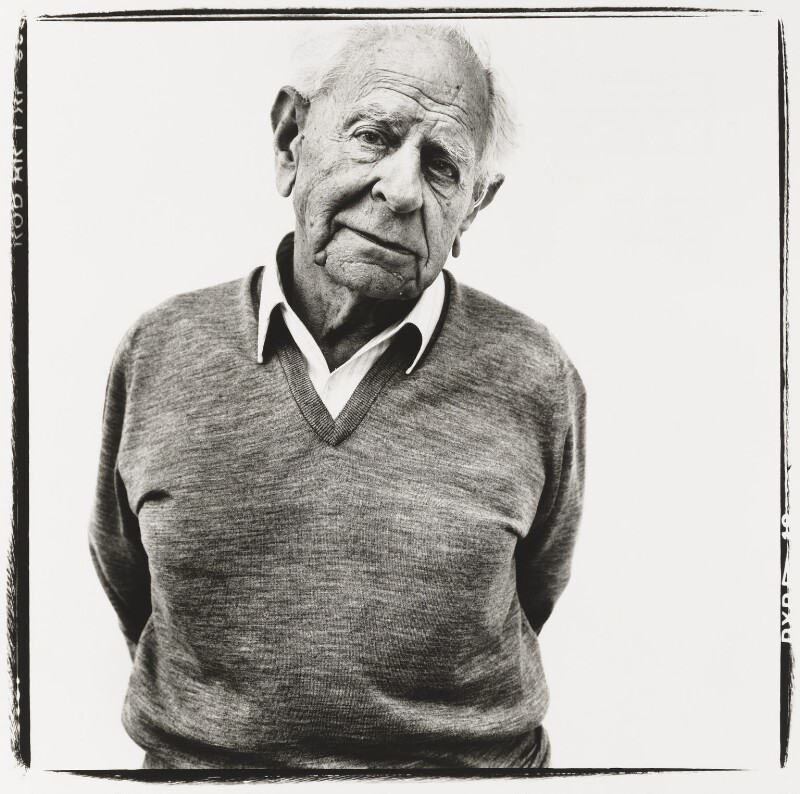
\includegraphics[width=0.5\textwidth]{images/karl-popper.png}

  \legend{Fonte: \href{https://www.npg.org.uk/collections/search/portrait/mw08238/Sir-Karl-Raimund-Popper?}{Steve Pyke}.}
\end{figure}

\hypertarget{secondary-section}{%
\section{Secondary section}\label{secondary-section}}

\begin{Shaded}
\begin{Highlighting}[numbers=left,,]
\CommentTok{\# library(datasets)}
\CommentTok{\# library(dplyr)}

\NormalTok{datasets}\SpecialCharTok{::}\NormalTok{iris }\SpecialCharTok{|\textgreater{}}
\NormalTok{  dplyr}\SpecialCharTok{::}\FunctionTok{as\_tibble}\NormalTok{() }\SpecialCharTok{|\textgreater{}}
\NormalTok{  dplyr}\SpecialCharTok{::}\FunctionTok{slice\_sample}\NormalTok{(}\AttributeTok{n =} \DecValTok{5}\NormalTok{) }\SpecialCharTok{|\textgreater{}}
\NormalTok{  gt}\SpecialCharTok{::}\FunctionTok{gt}\NormalTok{()}
\end{Highlighting}
\end{Shaded}

\hypertarget{tbl-iris}{}
\begin{longtable}{rrrrc}
\caption{\label{tbl-iris}A sample of the famous (Fisher's or Anderson's) iris data set }\tabularnewline

\toprule
Sepal.Length & Sepal.Width & Petal.Length & Petal.Width & Species \\ 
\midrule\addlinespace[2.5pt]
6.5 & 3.0 & 5.5 & 1.8 & virginica \\ 
6.5 & 3.0 & 5.8 & 2.2 & virginica \\ 
5.0 & 3.0 & 1.6 & 0.2 & setosa \\ 
5.0 & 3.5 & 1.6 & 0.6 & setosa \\ 
6.2 & 2.9 & 4.3 & 1.3 & versicolor \\ 
\bottomrule
\end{longtable}

\hypertarget{tertiary-section}{%
\subsection{Tertiary section}\label{tertiary-section}}

\begin{Shaded}
\begin{Highlighting}[numbers=left,,]
\CommentTok{\# library(datasets)}
\CommentTok{\# library(ggplot2)}

\NormalTok{ggplot2}\SpecialCharTok{::}\FunctionTok{ggplot}\NormalTok{(faithful, ggplot2}\SpecialCharTok{::}\FunctionTok{aes}\NormalTok{(}\AttributeTok{x =}\NormalTok{ eruptions, }\AttributeTok{y =}\NormalTok{ waiting)) }\SpecialCharTok{+}
\NormalTok{  ggplot2}\SpecialCharTok{::}\FunctionTok{geom\_point}\NormalTok{() }\SpecialCharTok{+}
\NormalTok{  ggplot2}\SpecialCharTok{::}\FunctionTok{xlim}\NormalTok{(}\FloatTok{0.5}\NormalTok{, }\DecValTok{6}\NormalTok{) }\SpecialCharTok{+}
\NormalTok{  ggplot2}\SpecialCharTok{::}\FunctionTok{ylim}\NormalTok{(}\DecValTok{40}\NormalTok{, }\DecValTok{110}\NormalTok{) }\SpecialCharTok{+}
\NormalTok{  ggplot2}\SpecialCharTok{::}\FunctionTok{geom\_density\_2d\_filled}\NormalTok{(}\AttributeTok{alpha =} \FloatTok{0.5}\NormalTok{) }\SpecialCharTok{+}
\NormalTok{  ggplot2}\SpecialCharTok{::}\FunctionTok{geom\_density\_2d}\NormalTok{(}\AttributeTok{linewidth =} \FloatTok{0.25}\NormalTok{, }\AttributeTok{colour =} \StringTok{"black"}\NormalTok{) }\SpecialCharTok{+}
\NormalTok{  ggplot2}\SpecialCharTok{::}\FunctionTok{theme}\NormalTok{(}\AttributeTok{legend.position =} \StringTok{"none"}\NormalTok{)}
\end{Highlighting}
\end{Shaded}

\begin{figure}[H]

\caption{\label{fig-eruption}Relationship between \emph{waiting time to
next eruption} (minutes) and \emph{eruption time} (minutes) at Old
Faithful Geyser, Yellowstone National Park, Wyoming, USA.}

{\centering 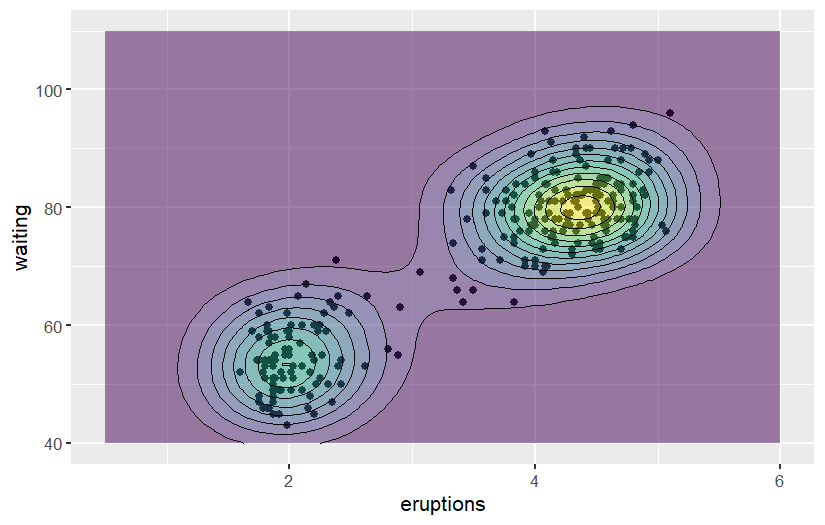
\includegraphics{index_files/figure-pdf/fig-eruption-1.png}

}

\end{figure}

\hypertarget{quaternary-section}{%
\subsubsection{Quaternary section}\label{quaternary-section}}

\begin{itemize}
\tightlist
\item
  Bullet point

  \begin{itemize}
  \tightlist
  \item
    Bullet point

    \begin{itemize}
    \tightlist
    \item
      Bullet point
    \end{itemize}
  \end{itemize}
\end{itemize}

\hypertarget{quinary-section}{%
\paragraph{Quinary section}\label{quinary-section}}

\begin{enumerate}
\def\labelenumi{\arabic{enumi}.}
\tightlist
\item
  List
\item
  List
\item
  List
\end{enumerate}

\bookmarksetup{startatroot}

\hypertarget{development}{%
\chapter{Development}\label{development}}

\begin{tcolorbox}[enhanced jigsaw, coltitle=black, colback=white, bottomrule=.15mm, breakable, titlerule=0mm, leftrule=.75mm, opacitybacktitle=0.6, colframe=quarto-callout-warning-color-frame, left=2mm, opacityback=0, toprule=.15mm, title=\textcolor{quarto-callout-warning-color}{\faExclamationTriangle}\hspace{0.5em}{Warning}, bottomtitle=1mm, toptitle=1mm, arc=.35mm, rightrule=.15mm, colbacktitle=quarto-callout-warning-color!10!white]

The text below is for demonstrative purposes only.

\vspace{0.25\baselineskip}

See \url{https://github.com/danielvartan/abnt} to learn more about this
template.

\end{tcolorbox}

Cillum qui eu non ipsum pariatur ad exercitation pariatur dolore veniam
amet cillum. Aliqua do nostrud aliquip in amet. Commodo sit tempor nulla
ipsum officia voluptate laborum elit minim proident Lorem. Id pariatur
reprehenderit non officia fugiat incididunt anim aliquip anim anim.
Ipsum irure magna quis est aute. Nostrud nulla mollit non labore. In
laboris mollit ea in. Excepteur eu do elit proident. Commodo tempor nisi
enim ex velit voluptate dolor mollit eiusmod in ullamco aliqua nostrud
id.

Eiusmod dolore sint proident consectetur reprehenderit exercitation
sunt. Nisi qui sit commodo anim consectetur in laborum dolore in labore
veniam labore commodo tempor. Sunt sit officia commodo quis magna.
Aliqua esse est adipisicing ea est ex esse esse officia sit culpa minim
amet dolore. Culpa dolore laborum sunt do commodo duis in velit. Mollit
duis voluptate aliquip magna labore aute sit dolore amet culpa labore.
Id tempor consectetur est anim ullamco ex nostrud voluptate excepteur.
Aliqua laboris aute laborum amet eu. Minim quis veniam et dolor quis
fugiat. Adipisicing amet est do aliqua nostrud amet excepteur ut.

\hypertarget{secondary-section-1}{%
\section{Secondary section}\label{secondary-section-1}}

Minim consectetur eu aliqua in elit incididunt labore amet consequat
cillum minim. Id sit duis duis ex velit proident mollit minim consequat
nulla. Aliqua elit do excepteur nulla nostrud exercitation nisi tempor
incididunt. Veniam dolore in non nisi veniam aliquip. Minim labore
excepteur ea est dolore laboris cillum. Laboris sit pariatur pariatur
veniam mollit nisi cupidatat qui qui quis laborum veniam dolor. Proident
aliquip do adipisicing dolor elit aute elit. Officia anim quis id
voluptate eu. Quis labore consectetur est magna. Laborum nulla ea non
Lorem officia aute.

\bookmarksetup{startatroot}

\hypertarget{conclusion}{%
\chapter{Conclusion}\label{conclusion}}

\begin{tcolorbox}[enhanced jigsaw, coltitle=black, colback=white, bottomrule=.15mm, breakable, titlerule=0mm, leftrule=.75mm, opacitybacktitle=0.6, colframe=quarto-callout-important-color-frame, left=2mm, opacityback=0, toprule=.15mm, title=\textcolor{quarto-callout-important-color}{\faExclamation}\hspace{0.5em}{Important}, bottomtitle=1mm, toptitle=1mm, arc=.35mm, rightrule=.15mm, colbacktitle=quarto-callout-important-color!10!white]

The text below is for demonstrative purposes only.

\vspace{0.25\baselineskip}

See \url{https://github.com/danielvartan/abnt} to learn more about this
template.

\end{tcolorbox}

Cillum qui eu non ipsum pariatur ad exercitation pariatur dolore veniam
amet cillum. Aliqua do nostrud aliquip in amet. Commodo sit tempor nulla
ipsum officia voluptate laborum elit minim proident Lorem. Id pariatur
reprehenderit non officia fugiat incididunt anim aliquip anim anim.
Ipsum irure magna quis est aute. Nostrud nulla mollit non labore. In
laboris mollit ea in. Excepteur eu do elit proident. Commodo tempor nisi
enim ex velit voluptate dolor mollit eiusmod in ullamco aliqua nostrud
id.

Eiusmod dolore sint proident consectetur reprehenderit exercitation
sunt. Nisi qui sit commodo anim consectetur in laborum dolore in labore
veniam labore commodo tempor. Sunt sit officia commodo quis magna.
Aliqua esse est adipisicing ea est ex esse esse officia sit culpa minim
amet dolore. Culpa dolore laborum sunt do commodo duis in velit. Mollit
duis voluptate aliquip magna labore aute sit dolore amet culpa labore.
Id tempor consectetur est anim ullamco ex nostrud voluptate excepteur.
Aliqua laboris aute laborum amet eu. Minim quis veniam et dolor quis
fugiat. Adipisicing amet est do aliqua nostrud amet excepteur ut.

\hypertarget{secondary-section-2}{%
\section{Secondary section}\label{secondary-section-2}}

Minim consectetur eu aliqua in elit incididunt labore amet consequat
cillum minim. Id sit duis duis ex velit proident mollit minim consequat
nulla. Aliqua elit do excepteur nulla nostrud exercitation nisi tempor
incididunt. Veniam dolore in non nisi veniam aliquip. Minim labore
excepteur ea est dolore laboris cillum. Laboris sit pariatur pariatur
veniam mollit nisi cupidatat qui qui quis laborum veniam dolor. Proident
aliquip do adipisicing dolor elit aute elit. Officia anim quis id
voluptate eu. Quis labore consectetur est magna. Laborum nulla ea non
Lorem officia aute.

% Back matter -----

\postextual

\addtocontents{toc}{\protect\vspace{1em}}
\begingroup
\renewcommand{\baselinestretch}{1}
\setcounter{footnote}{0}
\renewcommand{\thefootnote}{\fnsymbol{footnote}}
\printbibliography[heading=bay]
\endgroup

\cftinserthook{toc}{bibhook}
\addcontentsline{toc}{chapter}{
  \protect\numberline{}
  \newbibname
  \hspace{-0.25em}
}

\begin{apendicesenv}

\cleardoublepage
\phantomsection
\addcontentsline{toc}{part}{Appendices}
\appendix

\hypertarget{example}{%
\chapter{Example}\label{example}}

\begin{tcolorbox}[enhanced jigsaw, coltitle=black, colback=white, bottomrule=.15mm, breakable, titlerule=0mm, leftrule=.75mm, opacitybacktitle=0.6, colframe=quarto-callout-tip-color-frame, left=2mm, opacityback=0, toprule=.15mm, title=\textcolor{quarto-callout-tip-color}{\faLightbulb}\hspace{0.5em}{Tip}, bottomtitle=1mm, toptitle=1mm, arc=.35mm, rightrule=.15mm, colbacktitle=quarto-callout-tip-color!10!white]

The text below is for demonstrative purposes only.

\vspace{0.25\baselineskip}

See \url{https://quarto.org/docs/authoring/markdown-basics.html} to
learn about the basics of Markdown's syntax.

\end{tcolorbox}

Cillum qui eu non ipsum pariatur ad exercitation pariatur dolore veniam
amet cillum. Aliqua do nostrud aliquip in amet. Commodo sit tempor nulla
ipsum officia voluptate laborum elit minim proident Lorem. Id pariatur
reprehenderit non officia fugiat incididunt anim aliquip anim anim.
Ipsum irure magna quis est aute. Nostrud nulla mollit non labore. In
laboris mollit ea in. Excepteur eu do elit proident. Commodo tempor nisi
enim ex velit voluptate dolor mollit eiusmod in ullamco aliqua nostrud
id.

Eiusmod dolore sint proident consectetur reprehenderit exercitation
sunt. Nisi qui sit commodo anim consectetur in laborum dolore in labore
veniam labore commodo tempor. Sunt sit officia commodo quis magna.
Aliqua esse est adipisicing ea est ex esse esse officia sit culpa minim
amet dolore. Culpa dolore laborum sunt do commodo duis in velit. Mollit
duis voluptate aliquip magna labore aute sit dolore amet culpa labore.
Id tempor consectetur est anim ullamco ex nostrud voluptate excepteur.
Aliqua laboris aute laborum amet eu. Minim quis veniam et dolor quis
fugiat. Adipisicing amet est do aliqua nostrud amet excepteur ut.

\hypertarget{secondary-section-3}{%
\section{Secondary section}\label{secondary-section-3}}

Minim consectetur eu aliqua in elit incididunt labore amet consequat
cillum minim. Id sit duis duis ex velit proident mollit minim consequat
nulla. Aliqua elit do excepteur nulla nostrud exercitation nisi tempor
incididunt. Veniam dolore in non nisi veniam aliquip. Minim labore
excepteur ea est dolore laboris cillum. Laboris sit pariatur pariatur
veniam mollit nisi cupidatat qui qui quis laborum veniam dolor. Proident
aliquip do adipisicing dolor elit aute elit. Officia anim quis id
voluptate eu. Quis labore consectetur est magna. Laborum nulla ea non
Lorem officia aute.

\end{apendicesenv}

% -----
% Attachments (optional)
% -----

\begin{anexosenv}
\chapter{Example}

Lorem ipsum dolor sit amet, consectetur adipiscing elit. Pellentesque accumsan rutrum lacus, vitae iaculis nisi bibendum in. Nulla et pellentesque nisl. Proin mollis dui sit amet egestas fermentum. Maecenas eu odio odio. Aenean porta ipsum in mauris pharetra dapibus. Nunc dapibus libero nec dui lacinia, id ultricies lectus maximus. Mauris quis mauris in velit pulvinar rutrum. Cras congue ante in orci luctus placerat. Nullam sit amet nisi augue. Maecenas non ligula eros. Etiam nec dolor a mi bibendum auctor.

\clearpage

\includepdf{images/anx_1.pdf}
\end{anexosenv}

% % -----
% % Index (optional)
% % -----
%
% % Use `index: true` below the `format: pdf:` to activated this section.
% % See <https://quarto.org/docs/books/book-structure.html#creating-an-index>
% %   to learn more.
%
% \phantompart
% \printindex

\end{document}
